\documentclass{minimal}
\usepackage{tikz}
%% \usepackage{pgfmath}

\begin{document}

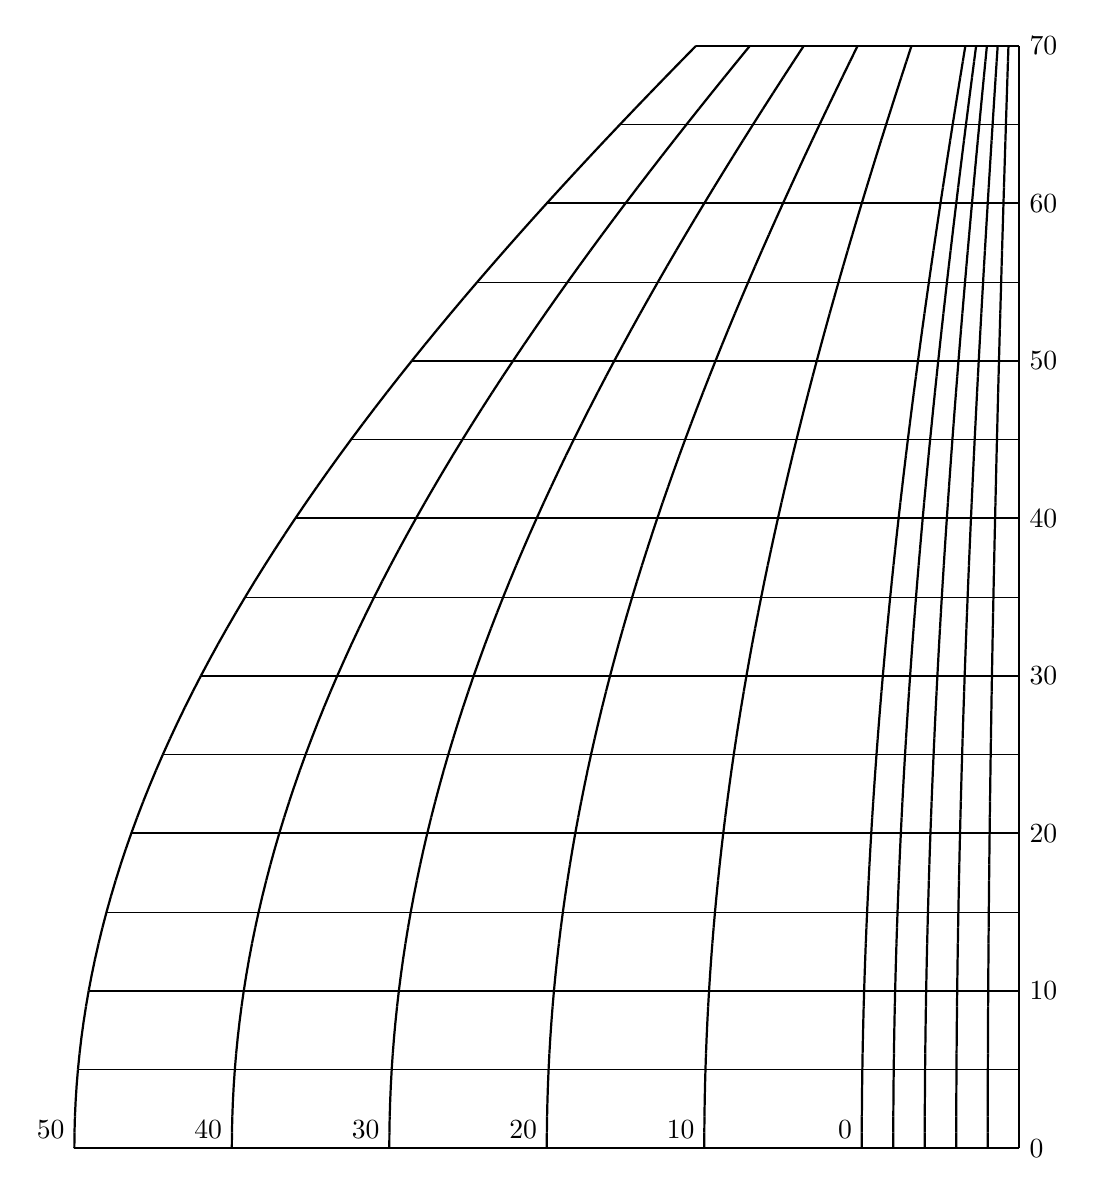
\begin{tikzpicture}[domain=0:60, scale=0.2]
  \foreach \y in {1,...,70} {   %for each degree in the vertical scale
    \foreach \step in {0,2,...,10,20,30,40,50,60} { %for each of the curved lines
      \draw[thick] ({sin(90-\y)*-\step+60},\y) -- ({sin(90-\y+1)*-\step+60},\y-1);
    }
  }
  \foreach \lat in {0,10,...,70} {  %For each of the horizontal latitude lines
    \draw[thick] ({sin(90-\lat)*-60+60},\lat) -- (60,\lat) node [right] {\lat};
  }
  \foreach \lat in {5,15,...,65} {  %For each of the thinner horizontal latitude lines
    \draw[ very thin] (60,\lat) -- ({sin(90-\lat)*-60+60},\lat);
  }
  \foreach \min in {0,10,...,50} {     %For each minute in the latitude scale (skip 0)
    \node [above left] at (50-\min, 0) {\min};
  }
\end{tikzpicture}

\end{document}
